\section{Introduction}

This is a security report created from your Kubernetes clusters protect by Carbon Black Container.

\section{Kubernetes clusters}

This is the list of Kubernetes clusters protected by Carbon Black Container.

\subsection{Kubernetes Clusters list}
\verbfile{./cluster_list.txt}

\subsection{Kubernetes Clusters diff}
This is the diff of new or removed Kubernetes clusters since last report:
\vskip10pt
\input{clusterlistdiff}

\section{Namespaces}

This is the list of \gls{ns} protected by Carbon Black Container.

\subsection{Namespaces list}
\verbfile{./namespace_list.txt}

\subsection{Namespaces list diff}
This is the list of new or removed namespaces since last report:
\vskip10pt
\input{namespacelistdiff}

\section{Container Registries}
\subsection{Container Registries list}
This is the list of container Registries detected by Carbon Black Container.
\vskip15pt

\verbfile{./registry_list.txt}

\vskip15pt

\subsection{Container Registries diff}
This is the diff of new or removed container Registries since last report:
\vskip10pt
%\verbfile{./registry_list_diff.txt}
\input{registrylistdiff}

\section{Hardening Policies}

This section list all security policies, and provides the number of exceptions and violations.

system & system & 0 & 6\\
\hline
demo & Any & 3 & 4\\
\hline
\end{tabular}


\begin{importantblock}
	Violations can be: alert or block or \gls{enforcement}. Modify your infrastructure to be compliant, and last option can be to add some exceptions.
\end{importantblock}

\section{Security alerts}

Carbon Black container provides 3 types of alerts:
\begin{enumerate}
  \item Containers Runtime alerts
  \item CB Analytics (Antivirus)
  \item Watchlists (IOCs: Feeds and custom Watchlists)
\end{enumerate}

\subsection{Containers Runtime alerts - Network}
\noindent

\input{runtimealert}
\vskip10pt

This is the list of Runtime security alerts, for more details, please see Carbon Black console.
\vskip10pt

\input{alertreason}

\begin{tipblock}
	Alerts can be reduced by increasing training period (1, 2, 7 days) or by restarting the training after a new deployment.
\end{tipblock}

\begin{importantblock}
	Port scan and malicious reputation should be investigated.
\end{importantblock}

\vskip10pt
\input{alertsremoteip}

\vskip10pt
\input{alertsnamespace}

\subsection{CB Analytics (NGAV - Next Gen Anti Virus)}
This section lists all virus detected at Runtime, in a container image or on the Linux node.

\subsection{Watchlists (EEDR - Enterprise Endpoint Detection and Response)}
This section lists all IOCs detected at Runtime, in a container image or on the Linux node.


\section{Malware and Secret Detection}
This section lists all virus and secrets detected in container images.

\input{malware}

\section{Vulnerabilities}
There's always vulnerabilities in all software.\\
The goal is to minimize the critical vulnerabilities (in Dark red)!

\newtcbox{\criticalvulncbox}{colframe=VCRITICAL,colback=VCRITICAL,top=0pt,bottom=0pt,colupper=white}
\newtcbox{\highvulncbox}{colframe=VHIGH,colback=VHIGH,top=0pt,bottom=0pt,colupper=white}
\newtcbox{\mediumvulncbox}{colframe=VMEDIUM,colback=VMEDIUM,top=0pt,bottom=0pt,colupper=white}
\newtcbox{\lowvulncbox}{colframe=VLOW,colback=VLOW,top=0pt,bottom=0pt}
\newtcbox{\unknownvulncbox}{colframe=VUNKNOWN,colback=VUNKNOWN,top=0pt,bottom=0pt,colupper=white}


\subsection{Vulnerabilities overview}
This is an overview of vulnerabilities in container images running in your Kubernetes cluster:

\input{vulnoverview}

%\subsection{Vulnerabilities histogram}
% 
%\pgfplotsset{compat=1.17}


\begin{figure}[htb]
  \centering
  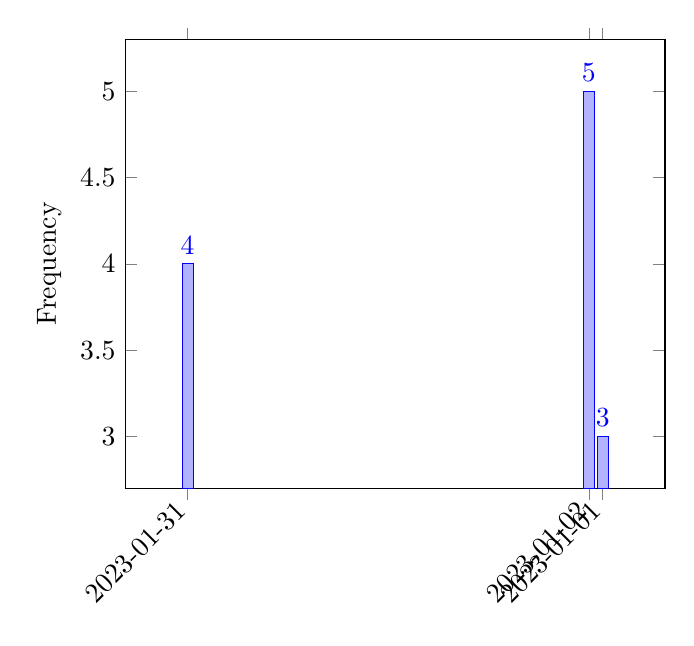
\begin{tikzpicture}
    \begin{axis}[
      ybar,
      bar width=0.8, % Adjust this value as needed
      enlargelimits=0.15,
      legend style={at={(0.5,-0.15)},
        anchor=north,legend columns=-1},
      ylabel={Frequency},
      xtick=data,
      xticklabels={
        2023-01-01, % replace with your actual dates
        2023-01-02,
        % ... Continue for the remaining days
        2023-01-31,
      },
      x tick label style={rotate=45, anchor=east},
      nodes near coords,
      nodes near coords align={vertical},
      ]
      % Replace the following data with your own for the last 31 days
      \addplot coordinates {
          (2023-01-01, 3) % Day 1
          (2023-01-02, 5) % Day 2
          % ... Continue for the remaining days
          (2023-01-31, 4) % Day 31
      };
    \end{axis}
  \end{tikzpicture}
  \caption{Histogram of the Last 31 Days}
  \label{fig:histogram}
\end{figure}


]

\subsection{Critical vulnerabilities}
Only container images with critical vulnerabilities will be listed below.


\vskip10pt

\tcbset{on line}
Color code:
\criticalvulncbox{Critical}
\highvulncbox{High}
\mediumvulncbox{Medium} 
\lowvulncbox{Low} 
\unknownvulncbox{Unknown} 

Example: 
\criticalvulncbox{200/100} = 
200 critical vulnerabilities / 100 critical vulnerabilities with a fix available.
\par

\begin{center}
\rule{0.5\linewidth}{1pt}
\end{center}

\subsection{default:dev}

gke.gcr.io
metrics-server

\criticalvulncbox{1/1}
\highvulncbox{8/8}
\mediumvulncbox{4/4}
\lowvulncbox{2/2}

\subsection{default:prod}

docker.io
vmwareallspark/acme-load-gen
latest
\criticalvulncbox{213/188}
\highvulncbox{1461/1198}
\mediumvulncbox{1794/1443}
\lowvulncbox{3434/2346}


gcr.io
vmwarecloudadvocacy/acmeshop-cart
1.0.0
\criticalvulncbox{62/7}
\highvulncbox{210/27}
\mediumvulncbox{187/27}
\lowvulncbox{10/4}


gcr.io
vmwarecloudadvocacy/acmeshop-order
1.0.1
\criticalvulncbox{56/7}
\highvulncbox{207/32}
\mediumvulncbox{184/29}
\lowvulncbox{7/5}


docker.io
tamirmich/log4j2-demo
0.0.3
\criticalvulncbox{46/6}
\highvulncbox{116/43}
\mediumvulncbox{84/20}
\lowvulncbox{6/3}


gcr.io
vmwarecloudadvocacy/acmeshop-front-end
rel1
\criticalvulncbox{38/4}
\highvulncbox{218/36}
\mediumvulncbox{173/31}
\lowvulncbox{11/9}


docker.io
weaveworksdemos/catalogue-db
0.3.0
\criticalvulncbox{30/26}
\highvulncbox{106/83}
\mediumvulncbox{113/74}
\lowvulncbox{7/5}


gcr.io
vmwarecloudadvocacy/acmeshop-payment
1.0.0
\criticalvulncbox{24/4}
\highvulncbox{133/29}
\mediumvulncbox{91/26}
\lowvulncbox{11/9}


docker.io
library/rabbitmq
3.6.8-management
\criticalvulncbox{23/19}
\highvulncbox{98/74}
\mediumvulncbox{152/78}
\lowvulncbox{9/6}


docker.io
weaveworksdemos/user-db
0.3.0
\criticalvulncbox{22/20}
\highvulncbox{103/80}
\mediumvulncbox{124/84}
\lowvulncbox{8/6}


gcr.io
vmwarecloudadvocacy/acmeshop-user
1.0.0
\criticalvulncbox{21/11}
\highvulncbox{81/23}
\mediumvulncbox{57/17}
\lowvulncbox{7/5}


docker.io
library/redis
5.0.3-alpine
\criticalvulncbox{14/2}
\highvulncbox{74/8}
\mediumvulncbox{48/14}
\lowvulncbox{7/4}


gcr.io
vmwarecloudadvocacy/acmeshop-catalog
rel1
\criticalvulncbox{14/4}
\highvulncbox{73/15}
\mediumvulncbox{56/16}
\lowvulncbox{6/4}


docker.io
openso/olivetin
latest
\criticalvulncbox{2/0}
\highvulncbox{16/4}
\mediumvulncbox{17/3}


docker.io
library/redis
alpine
\criticalvulncbox{2/0}
\highvulncbox{6/0}
\mediumvulncbox{6/0}
\lowvulncbox{1/0}



